\chapter{Prototype simulations and desing}
\chaptermark{Prototype simulations and desing}
\cleardoublepage
\minitoc
\section{Introduction}
\begin{refsection}
	\label{ch3:Introduction}
	In the previous chapter, we described different ways to measure a transverse beam profile. At \acrshort{ess}, both interceptive and non interceptive profilers will be installed along the accelerator. The beam profile will be also record on the target and upstream of the beam dump \cite{shea2013}. The interceptive measurements are mainly done with wire scanners. These devices cannot handle the incredible beam power of \acrshort{ess} at nominal conditions, and will be only used at low beam duty cycle \cite{Cheymol2013}. Therefore, Non invasive Profile Monitors, or \acrshort{npm}, will take over for higher beam power. The \acrshort{npm}s refers to two types of devices depending on the detection principle. Ionization Profile Monitors (\acrshort{ipm}) will be implemented exclusively in the cryogenic part of the accelerator whereas Fluorescence Profile Monitors (\acrshort{fpm}) are foreseen for all the remaining parts of the linac \cite{Thomas2016}. Our team is in charge of the design and the production of ten \acrshort{ipm}s. More information about the whole beam diagnostic framework at \acrshort{ess} is available in these documents \cite{Peggs2013,Shea:IBIC2017-MO2AB2}.

	The present chapter is dedicated to the studies and simulations performed in order to design the future \acrshort{ipm} for \acrshort{ess}. First, we would like to introduce and define the goals and requirements of this project, and why \acrshort{ipm} has been foreseen. Then, studies about the expected counting rate at \acrshort{ess} based on ionization cross section are presented. The different effects on profile is also presented in this chapter. Finally, the model of different readout is described with respect to previous conditions. For each study, the principle of each tool that has been used is briefly explained.

	\section{ESS requirements}
	This section is not the most exciting one but it still interesting to underline the different requirements and specifications that our devices should match. \acrshort{ess} has defined requirements for the whole machine, and they are organized on different levels from installation to subsystem. Every subsystems must meet each level of specifications. In the case of the \acrshort{npm} system, the most important are defined in the level 4 (beam instrument) and level 5 (non invasive profile monitor) requirements:
	\begin{itemize}
		\item The transverse beam profile shall be measured with a total measurement error in the $95\ \%$ energy extension of the beam of less than $\pm10\ \%$.
		\item The transverse beam profile shall be measured with a total measurement error in the RMS extension of the beam of less than $\pm10\ \%$.
		\item The transverse beam profile shall be measured with a spatial resolution of $\leq\ 0.05\ mm$.
		\item The devices shall be able to perform the measurements and report the relevant PV data at a repetition rate of $14\ Hz$.
		\item The transverse beam profile measurement shall have a dynamic range of $1000$.
	\end{itemize}

	Each cold \acrshort{npm} consists of a consecutive pair of \acrshort{ipm}s, each \acrshort{ipm} measuring a transverse direction. The pair is plugged in a specific vacuum vessel: the Linac Warm Unit. The design of the \acrshort{lwu} has been frozen just before the beginning of our project. In fact, the \acrshort{lwu} design is slightly different between one in Spoke section and one in Elliptical section. A pair of wire scanner is also mounted on the \acrshort{lwu}. The \acrshort{ipm}s should not encroach on the WS area, even if the wire scanners work low duty cycle whereas the \acrshort{ipm}s operate at higher duty cycle. The beam pipe aperture radius is respectively 50mm and 25mm for the Elliptical and the Spoke \acrshort{lwu}. We designed our detector to match with all the previous mechanical constraints.

	The \acrshort{ipm} will be in between two cryomodules in the cold part of the accelerator. The \acrshort{lwu} vessels itself are not cooled down however the superconducting cavities are closeby. The use of superconducting cavities imposes a moderately high vacuum and a clean environment. A too high pressure or a contamination may damage the cavities. An operating pressure of \(10^{-9}\ mbar\) is foreseen but the vacuum level may be even lower during the operation. The valves will be close by the safety unit if the pressure reach \(10^{-7}\ mbar\). Hence, our \acrshort{ipm} design must be compliant with a high vacuum level and particle free. Fig. \ref{chap3:LWU_Cryo} shows the \acrshort{lwu} vessel in between two cryomodules. On can see the two \acrshort{cf} 200 flanges and the two rectangular \acrshort{cf} flanges for the wire scanner.

	\begin{figure}[ht]
	% Changer l'image car pas à jours.
	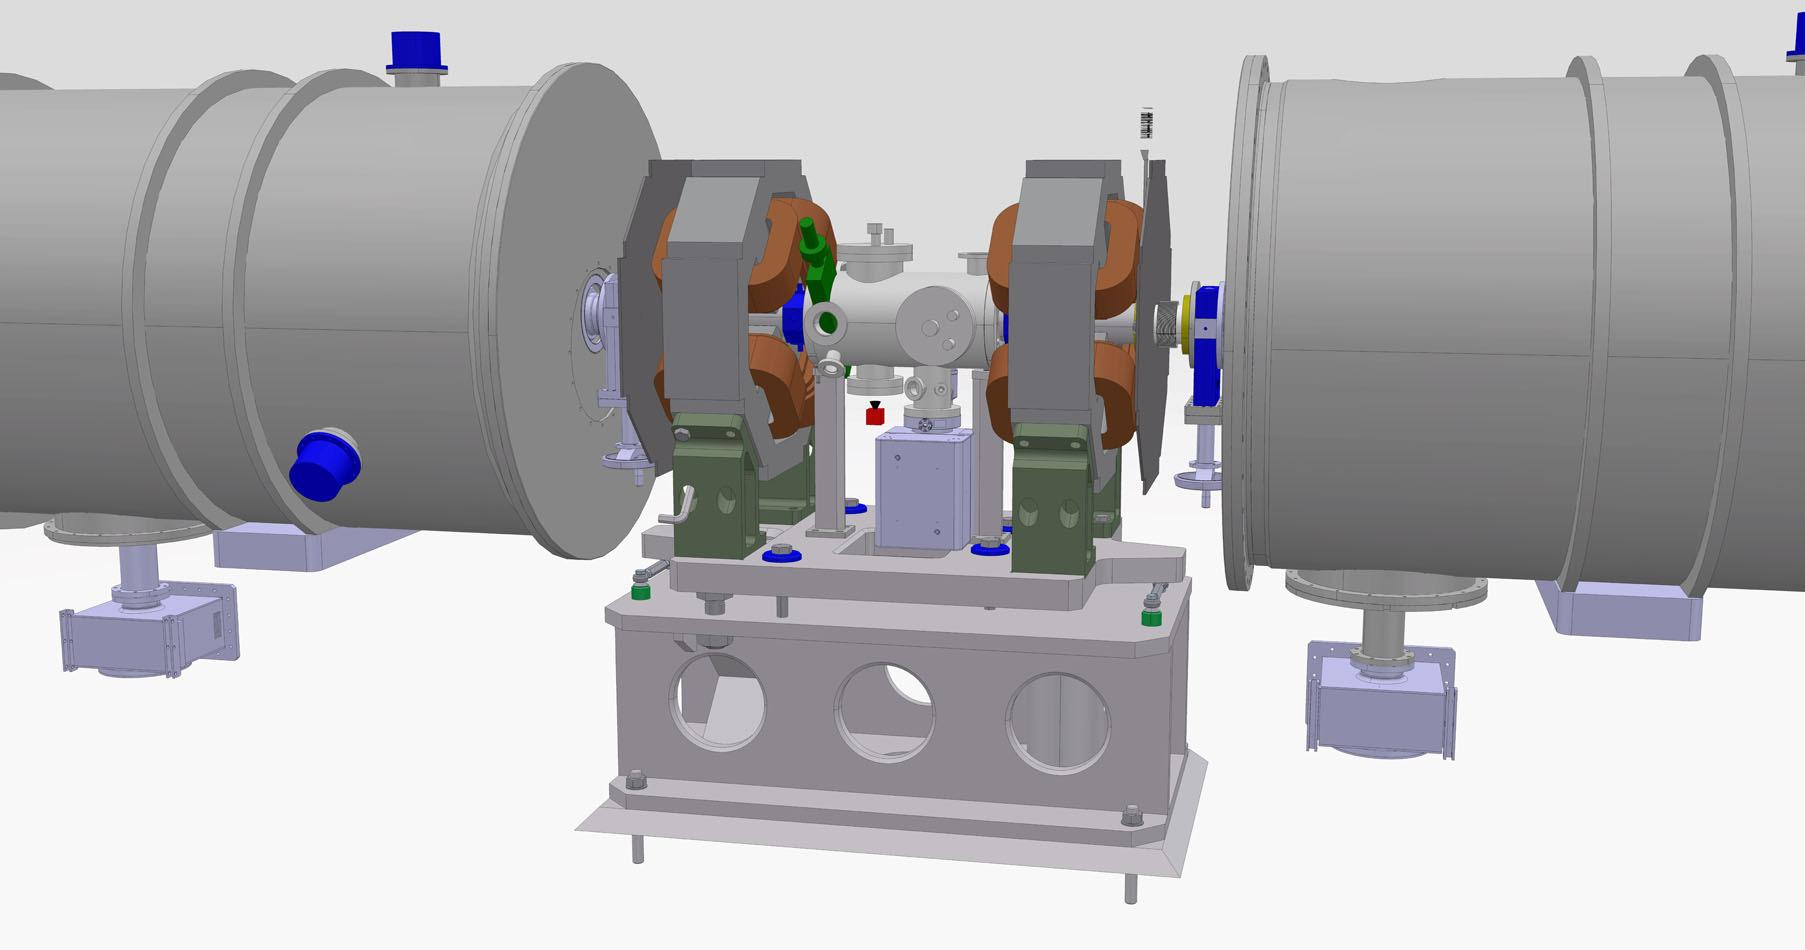
\includegraphics[width=\textwidth]{03_Prototype/figures/00_fig/fig016_LWU_Cryo.jpeg}
	\caption[The LWU vessel in between two quadrupole magnets and two cryomodules]{The LWU vessel in between two quadrupole magnets and two cryomodules. The IPMs will be mounted on the CF 200 flanges. \color{red}{[Changer l'image car elle n'est pas à jours ...]}}
	\label{chap3:LWU_Cryo}
\end{figure}


	\section{IPM simulations overview}
	As explained in the previous chapter, Ionization Profile Monitor (\acrshort{ipm}) is a type of non-destructive detector that measures the transverse profile of a beam (\acrshort{npm}).
	Principle of operation is summarized in the Figure \ref{chap3:ipm_outline} or in three main steps, as follows.
	Protons from beam pass through the vacuum, inducing ionizations of the residual gas: electron/ion pairs are created.
	Inside the \acrshort{ipm}, a strong electrical field drives electrons or ions towards a segmented readout plane.
	The profile is reconstructed in one transverse direction. For a complete profile a pair of \acrshort{ipm} is mandatory.

	\begin{figure}[!h]
	\centering
	\begin{subfigure}[t]{.45\textwidth}
		\centering
		\begin{tikzpicture}%[scale=1.3]
			% Variables
			% Ipm
			\pgfmathsetmacro{\LIPM}{1.8};
			\pgfmathsetmacro{\HIPM}{1.8};
			\pgfmathsetmacro{\TIPM}{0.1};
			% Deg
			\pgfmathsetmacro{\LDEG}{0.1};
			\pgfmathsetmacro{\HDEG}{0.3};
			\pgfmathsetmacro{\NDEG}{6};
			\pgfmathsetmacro{\SDEG}{1.5};
			\pgfmathsetmacro{\SPAND}{(2*\SDEG - \HDEG)/\NDEG}

			% Beam
			\draw[fill=blue!30] (0,0) circle (0.4) node[] {Beam};
			% Cage
			\draw (0,0) (-\LIPM,\HIPM)rectangle(\LIPM,\HIPM+\TIPM) node[above] {Anode};
			\draw (0,0) (-\LIPM,-\HIPM)rectangle(\LIPM,-\HIPM-\TIPM) node[below] {Cathode};
			\draw[fill=red!50] (-\LIPM/2,-\HIPM) rectangle(\LIPM/2,-\HIPM-\TIPM) node[midway,below] {Readout};
			% Ionized particle
			\draw[dashed,->] (0.1,0.1)--(0.1,\LIPM);
			\draw[dashed,->] (0.16,0.1)--(0.16,-\LIPM);
			\draw (0.1,0.15) node[blue] {$\bullet$};
			\draw (0.16,0.07) node[red] {$\bullet$};
			\draw[dashed,->] (-0.1,-0.2)--(-0.1,\LIPM);
			\draw[dashed,->] (-0.16,-0.2)--(-0.16,-\LIPM);
			\draw (-0.1,-0.15) node[blue] {$\bullet$};
			\draw (-0.16,-0.07) node[red] {$\bullet$};
			%Field
			\draw[->] (-1.2,1.5)--(-1.2,0.6) node [midway,right]{$\vec{E}$};
			% Degradors
			\foreach \x in {0,...,\NDEG}{
					\draw (0,0) (-\LIPM,\x*\SPAND - \SDEG) rectangle (-\LIPM+\LDEG,\x*\SPAND+\HDEG-\SDEG);
					\draw (0,0) (\LIPM,\x*\SPAND - \SDEG) rectangle (\LIPM-\LDEG,\x*\SPAND+ \HDEG-\SDEG);}
			%Profile
			\begin{axis}[every axis plot post/.append style={
							mark=none,domain=-3:3,samples=50,smooth},
					clip=false,
					axis y line=none,
					axis x line*=bottom,
					ymin=0,
					ymax=1,
					xtick=\empty,
					width=4cm,
					height=3cm,
					scale only axis,
					xshift=-2cm,
					yshift=-3.5cm
				]
				\addplot {\gauss{0}{0.3}{0.3}};
			\end{axis}
		\end{tikzpicture}
		\caption[How an IPM works]{How an IPM works. The electrical field can be reverted by inverting the polarity so it's possible to detect ions or electrons. Field correctors or degradors, on left and right, improve the field uniformity.}
		\label{fig:ipm_how}
	\end{subfigure}\hfill
	\centering
	\begin{subfigure}[t]{.45\textwidth}
		\centering
		%\includegraphics[width=0.9\linewidth]{01_Prototype/fig/proto.png}
		\caption[An IPM Prototype]{An IPM Prototype.
			The readout is visible through the rectangular slit, allowing ionization by-product passing through.
			Field correctors are also present on left and right plates.
		}
		\label{fig:ipm_proto}
	\end{subfigure}\hfill
	\caption[A conceptual view of an IPM and its implementation]{A conceptual view of an IPM and its implementation.}
	\label{fig:ipm}
\end{figure}


	Unfortunately, there is not framework that allows a full simulation of an \acrshort{ipm}. Each simulation step requires unique tools. In fact, most of the work consist of linking each simulation step together. The simulation can be split in three main categories same as the detector behaviour explained just above. In this chapter, we describe in the same order all the simulations and approximations that help us to design our detector.

	Firstly, the primary number of particle created by the proton beam should be evaluated, and it must sufficient in order to reconstruct a beam profile. However, this does not guaranteed that the primary particles reach the readout plane. Thus, it necessary to perform some electromagnetic simulations. Indeed, primary particle are sensitive to the non uniformities of the extraction field, and space charge effect induced by beam. These effects may disturb the profile measurements or reduce the number of primary particles. Therefore, they should be quantified. Lastly, the signal creation in the readout device should be evaluated with respect to previous simulations. The response of the readout mainly depends on its type.

	\section{Particle through matter}
	%TODO: Finir
	The interactions of particles with matter are an important aspect of nuclear or particle detection \cite{Knoll2010,Leo1994}. A particle will lose energy when it passes through a medium. The physical process behind the energy transfer mainly depends on the characteristics of the particle. These topics has been studied and improved over the last century. It often combines complicated theoretical laws with approximations or empirical models. This topic is very wide, hence in the following only the meaningful information will be described.

	As explained before, the \acrshort{ipm}s rely on the collection of the ionized residuals gas. The number of ionized particles is important since it will give the minimum sensitivity needed by the readout to measure a profile. First, we need to know how many particles are created by the beam itself along the vacuum residual gas. Then we should understand how theses secondary particles create signal in the sensitive part of our \acrshort{ipm}.


	\subsection{Interaction of charged particles with matter}
	%TODO: Finir
	For heavy charged particles, the main interaction is due to electromagnetic interactions of the incident particle with the orbiting electrons of the medium. A particle is considered heavy if its mass is far higher than the mass of an electron. The incident particle will transfer a small amount of its energy to an electron of the medium at each electronic collision. In 1930 Bethe proposed an equation that describes the mean rate of energy losses per distance of a heavy charged particle \cite[]{Bethe1930}. The so-called Bethe equation derives from the coulomb interactions. The equation has been improved over year \cite{Bloch1933,Fermi1940,Fano1963}. The expression of the linear stopping power for heavy charged particle is defined by the following equation \cite[p. 446]{Tanabashi2018}:
	\begin{equation}
		- \bigg \langle \frac{dE}{dx} \bigg \rangle =K \rho \frac{Z}{A} \frac{z^{2}}{\beta^{2}} \left[\frac{1}{2} ln \left(\frac{2 m_{e} \beta^{2} \gamma^{2} T_{max}}{I^{2}} \right) - \beta^{2} - \frac{\delta(\beta \gamma)}{2} - \frac{C}{Z} \right]
	\end{equation}

	\(K\) is a constant factor defined by \(K=4 \pi N_{a} r_{e}^{2} m_{e} c^{2}\) where \(m_{e}\) is the classical electron radius. For convenience, the stopping power is usually expressed in \(MeV/cm\). In this case, \(K\) is equal to \(0.307075\).

	Other terms in the bethe equation can be dissociated in two group. First, the incident particle related terms. The maximum transfer energy for one collision is given by the following equation:
	\begin{equation}
		T_{max} = \frac{2 m_{e} \beta^{2} \gamma^{2}}{1 + \frac{2 \gamma m_{e} }{M} + \left( \frac{m_{e}}{M} \right)^{2}}
	\end{equation}
	Where, \(M\) and \(m_{e}\) are respectively the incident particle and electron mass. The \(\beta\) and \(\gamma\) variables have their normal significance of the Lorentz factors.

	Finally, the terms related to medium. \(Z\), \(A\) and rho are respectively the atomic number, the mass number and the density of the given medium. In most of case the \(\frac{Z}{A}\) ratio is close to \(0.5\) except when a medium contains hydrogen. Sometime, Bethe equation is given independently from the density.
	The mean excitation energy \(I\) is the only non trivial variable in the Bethe equation \cite{Berger1984,Berger1993}. The computation is quite heavy because it requires to measurement  the oscillator strength for each material. Table \ref{chap3:WandI} gives the \(I\) value for common material.

	Two correction factors are often used to improve the accuracy of the Bethe equation at low and high energies. The density effect \(\frac{\delta(\beta \gamma)}{2}\) corrects the effects at relativistic energies \cite{Sternheimer1984}. The shell correction \(\frac{C}{Z}\) improves the accuracy at low energies \cite{Bichsel2002}.

	\begin{figure}[ht]
	\includesvg[width=\textwidth]{03_Prototype/figures/00_fig/fig001_bethe_2}
	\caption[Typical mass stopping power plot for protons]{Typical mass stopping power plot for protons. Here the mass stopping is plotted for proton in hydrogen and nitrogen.The calculation was done with respect to the Bethe formula and has been crosschecked with NIST PSTAR table which contains both computed and experimental values \cite{Seltzer1993}. The Bethe equation gives between \(0.2\ <\ \beta\gamma\ <\ 100\). However at lower and higher energies the Bethe formula is no more reliable.}
	\label{chap3:bethe1}
\end{figure}


	Fig. \ref{chap3:bethe1} shows the mass stopping power of a proton in two different mediums. The blue region represents the energy range of protons in the cryogenic part of \acrshort{ess}, where \acrshort{ipm}s will be located. One can see that the minimum of energy loss is reach at 2 GeV.

	The Bethe model has been tested show good agreement with experimental data. However, at very low or high energies the Bethe equation is no more usable. In these regions specific models are used to describe the energy loss in matter.

	The Bethe model is also not compatible with low mass particles like electrons and positrons. The Bethe must be modified for these particles \cite{Rieke1972}\cite[p. 452]{Tanabashi2018}. At low energies, electrons lose its energy by ionization like ion. Whereas at energies above few MeV, electrons also lose energy through bremsstrahlung radiation.

	\subsection{Electron ion pairs production}
	%TODO: Finish
	We just defined the mean energy loss rate of a charged particle per unit of distance. When a particle pass through a medium it may deposit its energy to an electron of the medium atoms.
	If the energy is sufficient an ionization happens: an electron is ejected from the electronic shell leading to an creation of an ion and a electron. In case of molecule, the ionization process may be dissociative i.e. it may break the molecular bound. The cross section for dissociative ionization is far lower than the one for pure ionization \cite{Dimopoulou2004}.

	By introducing W, the average energy to produce a ion electron pair in a medium, it is possible to estimate the number of ion/electron pairs created for a given detector length \cite[]{Weiss1955,Bichsel1979}.

	\begin{equation}
		N_{electrons}= \frac{\big \langle \frac{dE}{dx} \big \rangle}{W_{n}} \Delta x
	\end{equation}

	When an electron is ejected it has a certain probability to ionize other atoms if its energy is enough. These secondary electrons are called delta rays or delta electrons. This phenomena becomes rare and negligible when the medium has very low density like in a vacuum system. The W parameter includes the delta ray electrons, hence the W value is biased for us since our detectors work at very low pressure \cite[p. 470]{Tanabashi2018}. Table \ref{chap3:WandI} gives, as example, the W values for several materials.

	\begin{table}[ht]
	\centering
	\caption[Mean excitation energie, average energy to produce a pair and density values for severals mediums at Normal Temperature and Pressure (NTP)]
	{Mean excitation energie, average energy to produce a pair and density values for severals mediums at Normal Temperature and Pressure (NTP). Complete reviews of \(I\) and \(W\) values are available in \cite{Kamakura2006}\cite{Bichsel1979}.}
	\label{chap3:WandI}
	\begin{tabular}{llll}
		\toprule
		Gas        & \(I\) (\(\mathrm{eV}\)) & \(W\) (\(\mathrm{eV}\)) & \(\rho\) (\(\mathrm{kg/m^{3}}\)) \\
		\midrule
		\(H_{2}\)  & \(18.8\)       & \(36.43\)  &  \(0.0899\)  \\
		\(CO\)     & \(85.9\)       & \(34.5\)   &  \(1.165\)  \\
		\(CO_{2}\) & \(85.00\)      & \(34.21\)  &  \(1.842\)  \\
		\(N_{2}\)  & \(82.00\)      & \(36.39\)  &  \(1.165\)  \\
		\bottomrule
	\end{tabular}
\end{table}

	When the medium is a mixture of several compounds then it is necessary to calculate the mean stopping power for each of them with respect to their mass proportions:
	\begin{equation}
		N_{total}= \sum_{n= First}^{Last} N_{compound\ n}= \sum_{n= First}^{Last} w_{n} \frac{\big \langle \frac{dE}{dx}\left(\rho_{n},I_{n},A_{n},Z_{n}\right) \big \rangle}{W_{n}} \Delta x
	\end{equation}
	The calculation can be done for each single element or for each molecule in the compound.
	However, the second computation is preferable since the \(I\) values are in general higher for molecules \cite[p. 451]{Tanabashi2018}.

	\subsection{Calculation}

	Now that we defined all the physic background, we should be able to estimate the number of primary particles that will be created in the \acrshort{ess} conditions. We tried two different approaches: naive computation of Bethe equation and simulations through a framework.

	The Bethe formula is easy to implement since it require to know only the composition of the medium and the \(I\) value of each compound. The expected pressure in the cryogenic part at \acrshort{ess} is around \(10^{-9}\ mbar\), and the gas composition is given in Table \ref{chap3:ess_vacuum_gas}.

	\begin{table}[ht]
	\centering
	\caption[Expected residual vacuum gas in the cold part of ESS Linac, provided by ESS vacuum group]
	{Expected residual vacuum gas in the cold part of ESS Linac, provided by ESS vacuum group.}
	\label{chap3:ess_vacuum_gas}
	\begin{tabular}{llll}
		\toprule
		Gas        & Mass percentage (\(\%)\) & $p_{i}$ (\(\mathrm{mbar}\)) & $\rho_{i}$ $(\mathrm{g/cm^{3}}$) \\
		\midrule
		\(H_{2}\)  & \(79\)          & \(7.9 10^{-10}\)   & \(6.52\cdot
		10^{-17}\)                                                                \\
		\(CO\)     & \(10\)          & \(1.0 10^{-10}\)   & \(1.15\cdot
		10^{-16}\)                                                                \\
		\(CO_{2}\) & \(10\)          & \(1.0 10^{-10}\)   & \(1.8\cdot
		10^{-16}\)                                                                \\
		\(N_{2}\)  & \(1\)           & \(1 10^{-11}\)     & \(1.14\cdot
		10^{-17}\)                                                                \\
		\bottomrule
	\end{tabular}
\end{table}

	We suppose that the residual gas follows the perfect gas law. We also assume that the linear density scaling of Bethe equation remains true in high vacuum \cite[p. 446]{egber2012}\cite{Ishimaru1995}. Hence, the partial pressure and the density for each gas is calculated with respect to the previous pressure. The primary signal is computed at \acrshort{ess} nominal conditions given in Table [la table chapitre sera dans le chapitre précédent].

	Fig. \ref{chap3:ess_primary_particles} shows the number of electron ion pairs created for each gas species versus the \acrshort{ess} range of energies. The different \acrshort{ipm}s locations is marked by a blue line. One can see that the density has a strong influence on the primary signal. Although the hydrogen is the main species in term of proportion, its contribution to primary signal is close to the one from carbonate species. As explained just before, the W value may overestimate the number of pairs created due to secondary delta rays.

	\begin{figure}[ht]
	\includesvg[width=\textwidth]{03_Prototype/figures/00_fig/fig015_ess_primary_particle}
	\caption[]{Typical mass stopping power plot.}
	\label{chap3:ess_primary_particles}
\end{figure}


	[J'ai essayé de faire les comparaisons avec garfield mais les résultats sont étranges. Francesca a les même soucis. En cours d'investiguation]
	[MAJ: Le bug a été corriger par l'équipe de Garfield. Ils vont également regarder en détail les processus. Mais je dois refaire les plots. ]

  \begin{table}[ht]%{r}{0.5\textwidth}
	\centering
	\caption[Comparison of expected number of electrons between calculation using Bethe equation and results from Garfield++.]
	{Comparison of expected number of electrons between calculation using Bethe equation and results from Garfield++}
	\label{chap3:GarfieldBethe}
	\begin{tabular}{llll}
		\toprule
		Energy    & \(N_{Bethe}\) & \(N_{garfield}\) & Factor \\
		\midrule
		\(97.2\)  & \(100210\)    & \(52537\)             & \(0.52\)   \\
		\(231.4\) & \(54970\)     & \(27463\)             & \(0.50\)   \\
		\(278.9\) & \(49160\)     & \(26124\)             & \(0.53\)   \\
		\(315.8\) & \(45850\)     & \(23769\)             & \(0.52\)   \\
		\(628.3\) & \(33600\)     & \(17522\)             & \(0.52\)   \\
		\bottomrule
	\end{tabular}
\end{table}

	\subsection{Pressure uniformity}
	[Simulation molflow: j'avais il y a longtemps regarder l'uniformité de la préssion dans l'enceinte. Je sais pas si c'est vraiment utile]

	\section{Profile distortion effects}

  \section{Extraction field}
  The IPMs can be seen as a parallel plate detector. In an ideal IPM these plates are infinite sized. The extraction field is then completely oriented in a single direction, normal to the detection plane. So the projection of the profile is perfect on this plane. In reality, the plates can not be considered infinite sized because the distance between the two electrodes is equal to the gap size between them. In these conditions the field is no more uniform for several reasons including:
  \begin{itemize}
    \item The effects induced by the sides of the cage are no longer negligible. Uniformity is strongly influenced by the peak effects of the plates.
    \item The geometry of the vacuum chamber has also some influences on the field uniformity. Indeed the vacuum chamber is considered to be at ground. Walls close to the IPMs will change the electric field lines inside the IPMs.
    \item The way to create the field with high voltage power supplies. We will see later that some readouts can only work in certain configurations of high voltages.
  \end{itemize}
  The non-uniformity of the electric field is very problematic because it prevents the correct measurement of the beam profile. It also determines the maximum size of the detection area which must be in a zone as uniform as possible. To overcome all these effects, several solutions can be considered. 

	\subsection{Maxwell equations at steady state}
	\begin{align}
		 & \overrightarrow{\nabla} \cdot \overrightarrow{E} = \frac{\rho}{\epsilon_{0}}                                            \\
		 & \overrightarrow{\nabla} \times \overrightarrow{E} = - \frac{\partial \overrightarrow{B}}{\partial t}                    \\
		 & \overrightarrow{\nabla} \cdot \overrightarrow{B} = 0                                                                    \\
		 & \overrightarrow{\nabla} \times \overrightarrow{B} = \overrightarrow{J} + \frac{\partial \overrightarrow{E}}{\partial t}
	\end{align}

	\subsection{Solving poisson equation}
	[Poisson]
	\begin{equation}
		\Delta V = \overrightarrow{\nabla}^{2}V = -\frac{\rho}{\epsilon_{0}}
	\end{equation}

	[FDM]
	\begin{align}
		 & f(x+h) = f(x)+hf^{\prime}(x)
		+\frac{h^2}{2}f^{\prime\prime}(x)+\frac{h^3}{6}f^{\prime\prime\prime}(x) + O(h^{4}) \\
		 & f(x-h) = f(x)-hf^{\prime}(x)
		+\frac{h^2}{2}f^{\prime\prime}(x)-\frac{h^3}{6}f^{\prime\prime\prime}(x) + O(h^{4})
	\end{align}

	\begin{equation}
		f^{\prime\prime}(x) = \frac{f(x+h) + f(x-h) - 2f(x)}{h^{2}} + O(h^{2})
	\end{equation}

	\begin{equation}
		\begin{split}
			h^{2}f^{\prime\prime}(x,y)=&f(x+h,y) + f(x-h,y) \\
			+ &f(x,y+h) + f(x,y-h) \\
			- 4&f(x)+ O(h^{2})
		\end{split}
	\end{equation}

	\begin{align}
		Id \cdot E_{u} + & A \cdot E_{c} = D                  \\
		Id \cdot E_{u} + & A \cdot E_{c} + Id \cdot E_{d} = D \\
		                 & A \cdot E_{c} + Id \cdot E_{d} = D
	\end{align}

	\begin{equation}
		A =
		\begin{pmatrix}
			-4      & 1      & 0      & \cdots \\
			1      & -4      & 1      & \cdots \\
			0      & 1      & -4      & \cdots \\
			\vdots & \vdots & \vdots & \ddots
		\end{pmatrix}
	\end{equation}

	\begin{equation}
		\begin{bmatrix}
			A      & Id     & 0      & \cdots \\
			Id     & A      & Id     & \cdots \\
			0      & Id     & A      & \cdots \\
			\vdots & \vdots & \vdots & \ddots
			\cdot
		\end{bmatrix}
		\begin{bmatrix}
			E \\
			E \\
			E \\
			E
		\end{bmatrix}
		=
		\begin{bmatrix}
			D \\
			D \\
			D \\
			D
		\end{bmatrix}
	\end{equation}

	[FEM]
	\begin{align}
		\int_{\Omega}^{} \varphi \Delta v d\Omega                                                                             & = \int_{\Omega}^{} \varphi f d\Omega \\
		\int_{\Omega}^{} \vec{\nabla} \varphi \cdot \vec{\nabla} v - \int_{d\Omega}^{} \varphi \vec{\nabla} v \cdot n d\Sigma & = \int_{\Omega}^{} \varphi f d\Omega
	\end{align}

	\begin{align}                                                      \\
		 & \int_{\Omega}^{} \vec{\nabla} \varphi \cdot \vec{\nabla} v = \int_{\Omega}^{} \varphi f d\Omega + \int_{d\Omega}^{} \varphi \vec{\nabla} v \cdot n d\Sigma
	\end{align}

	[BEM]

	[J'ai demandé aux gens de COMSOL ce qui expliquer les différences entre BEM et FEM dans COMSOL]

	\begin{figure}[!h]
	\begin{subfigure}{.5\textwidth}
		\centering
		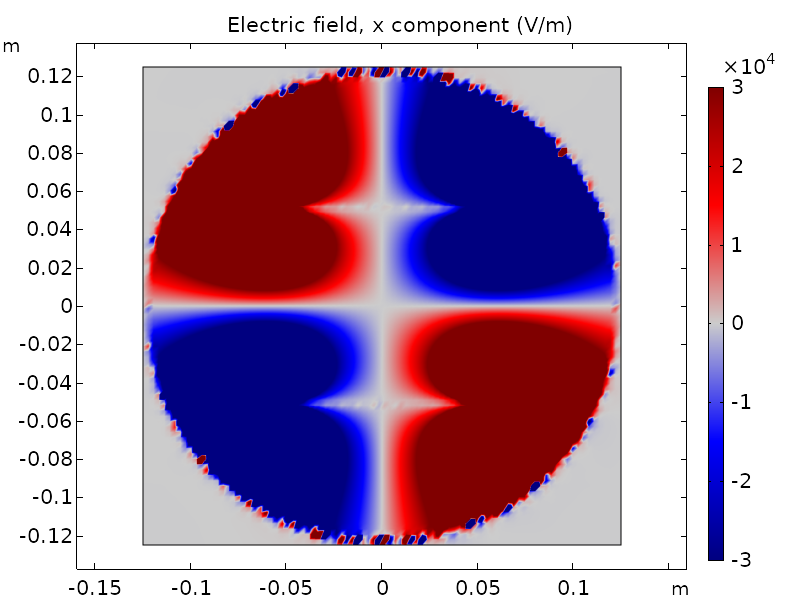
\includegraphics[width=\textwidth]{03_Prototype/figures/00_fig/fig012_BEMa.png}
		\caption{}
		\label{}
	\end{subfigure}\hfill
	\begin{subfigure}{.5\textwidth}
		\centering
		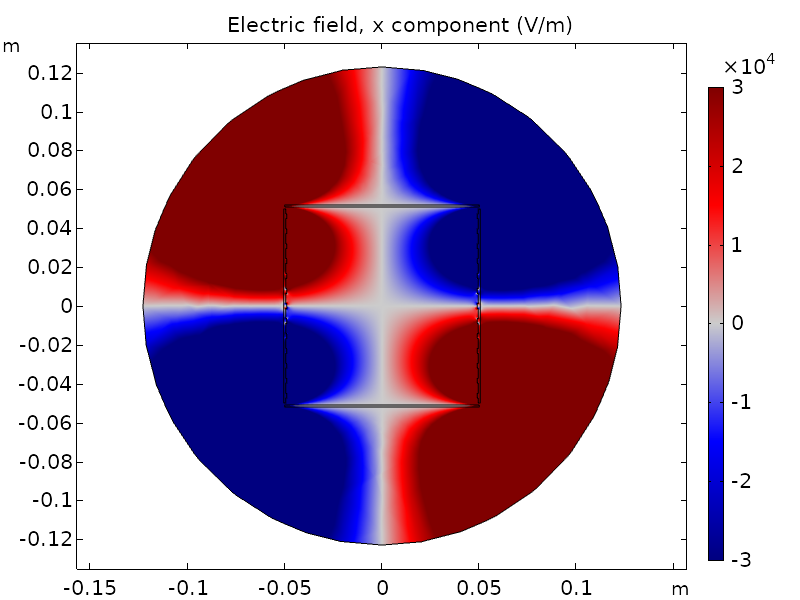
\includegraphics[width=\textwidth]{03_Prototype/figures/00_fig/fig012_FEMa.png}
		\caption{}
		\label{}
	\end{subfigure}
	\vskip\baselineskip
	\begin{subfigure}{.5\textwidth}
		\centering
		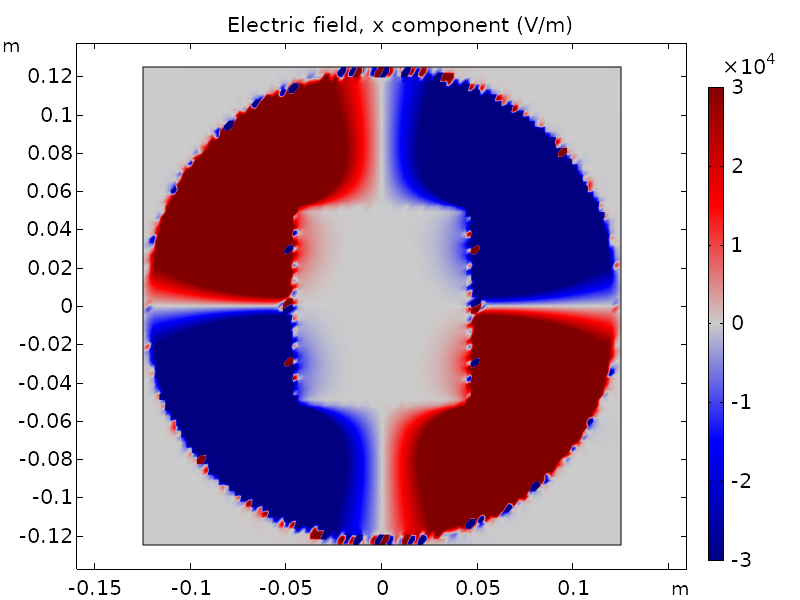
\includegraphics[width=\textwidth]{03_Prototype/figures/00_fig/fig012_BEMb.png}
		\caption{}
		\label{}
	\end{subfigure}\hfill
	\begin{subfigure}{.5\textwidth}
		\centering
		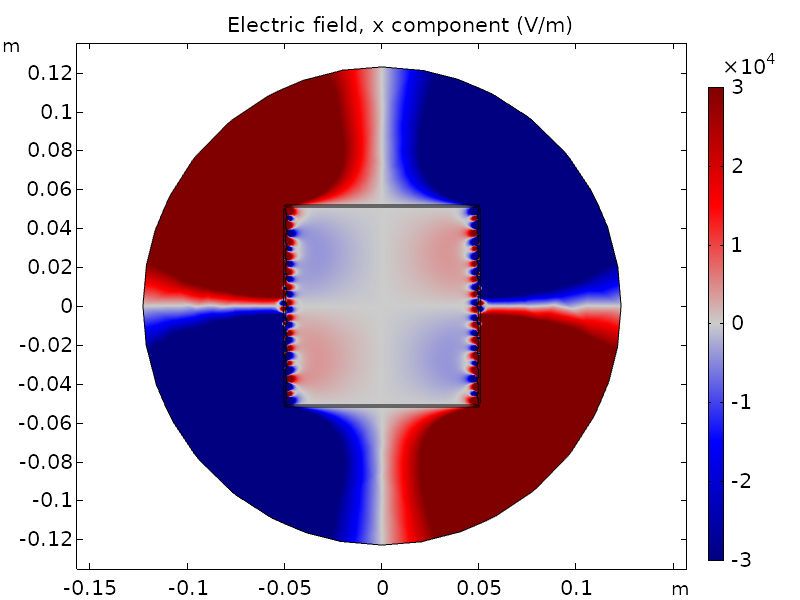
\includegraphics[width=\textwidth]{03_Prototype/figures/00_fig/fig012_FEMb.png}
		\caption{}
		\label{}
	\end{subfigure}
	\caption[]{}
	\label{chap3:FEMvsBEM}
\end{figure}


	\subsection{COMSOL}
	COMSOL is proprietary all-in-one multi-physic simulation software able to solve various problems from structural mechanical analysis to optical raytracing \cite{comsol2018}. We use COMSOL with the AC/DC module to simulate the static electrical field in the \acrshort{ipm} box \cite{comsolacdc2018}. COMSOL allows to quickly define, simulate and post process physical model like its competitors \cite{cststudio2018,ansys2018,couloumb2018}. The typical workflow is divided in three main steps.

	The first step is to implement the detector geometry into COMSOL. The software includes basic \acrshort{cad} features that allows to quickly create two or tridimensional geometries. The users can directly import a mesh from file generated by external \acrshort{cad} tools. However, importing from \acrshort{cad} often increases the model complexity and so the simulation time and it is much faster to directly implement the geometry with COMSOL.  In our case, only the inner shape of the vacuum chamber and the \acrshort{ipm}s must be defined. All other conductive bodies that enclose the vacuum are not relevant for an electrostatic simulation. Therefore, the geometry can be simplified. Fig. \ref{chap3:COMSOL_LWU} shows, on the left, a 3D drawing of the \acrshort{ess} vacuum vessel with the two \acrshort{ipm}s within. And on the right, an example of the simplified geometry implemented in COMSOL.

	\begin{figure}[ht]
	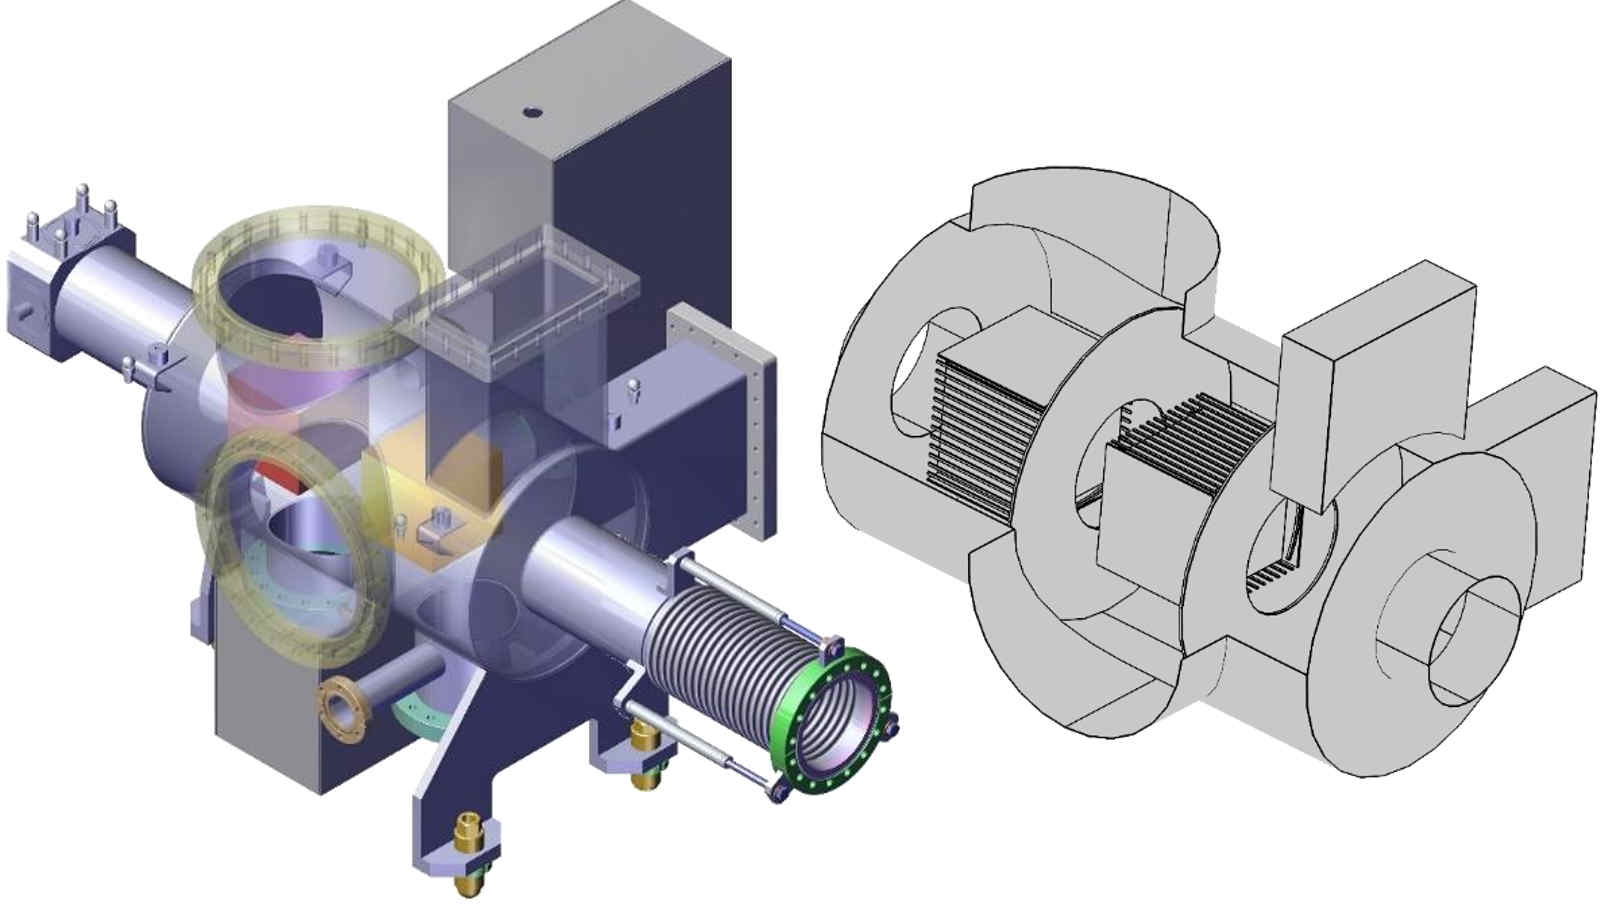
\includegraphics[width=\textwidth]{03_Prototype/figures/00_fig/fig003_COMSOL_LWU.jpeg}
	\caption[Typical mass stopping power plot]{Typical mass stopping power plot.}
	\label{chap3:maxwell_gas_log1}
\end{figure}


	The next step consists on the discretization of the previous geometry in many Lagrange elements in order to form a mesh. Fig. \ref{chap3:COMSOL_meshing_elements} shows main meshing elements available in COMSOL. For an electrostatic tridimensional study, COMSOL uses quadratic tetrahedral elements by default. The meshing algorithm tries to create elements that fit well to geometry. So, if a geometry has small parts then the size of elements will be reduced in these regions. Conversely, mesh cells will become bigger and bigger in coarse regions of the geometry. However, this behavior is not desirable for us. Indeed, in an \acrshort{ipm}, the region of interest has no geometrical variation consequently mesh element are particularly big there. This may lead to inaccurate results. Fortunately, the user can change the characteristics and the nature of the elements in specific region of the defined geometry. We used a tetrahedral mesh apart from the \acrshort{ipm} box where a cubic mesh with high granularity is defined. The meshing step is very memory consuming and a poorly optimized mesh may destroy performance.

	\begin{figure}[ht]
	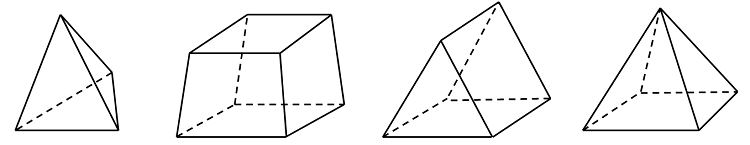
\includegraphics[width=\textwidth]{03_Prototype/figures/00_fig/fig006_COMSOL_meshing_elements.png}
	\caption[3D Mesh elements included in COMSOL]{Mesh elements included in COMSOL software. COMSOL uses tetrahedral elements by default to mesh a 3D geometry.}
	\label{chap3:maxwell_gas_log1}
\end{figure}


	The last step is to define boundary conditions. COMSOL hides completely the mathematical aspect of the \acrshort{fem} and directly express the boundary conditions in a physical meaning. In AC/DC module is mainly consist of defining fixed potentials or charge densities. A more detailed description of each boundary condition type can be found in the reference manual. COMSOL is able to solve electrostatic problems by means of \acrshort{fem} or \acrshort{bem} since version 5.3a.
	Once solved, the problem can be processed directly in COMSOL. Data can be also exported to an external file in text format (column separated values or VTU format).

	To conclude, we would like to introduce all the relevant assumptions made in our COMSOL model. All conductors and insulators are supposed to be perfect. Field correctors and electrodes are thicker than reality since it is not feasible to describe a micrometer deposition layer in a meter scale simulation. The resistor chain at the back of field corrector is not implement as well as the connection wires, feedthroughs and connectors. The vacuum vessel is supposed to be at the same ground as power supplies, and without any charge on its surface.

	\subsection{Criteria}

	\begin{equation}
		\bar{\vec{E}} = \frac{\sum_{i=1}^{N}\sqrt{\vec{E}_{i}^{2}}}{N}
	\end{equation}

	Particles are released and we observed the drift in the field cage due to lorentz force:

	\begin{equation}
		\vec{F} = m \cdot a = q \cdot (\vec{E}(\vec{r},t) + \vec{v} \times \vec{B}(\vec{r},t))
	\end{equation}

	First initial position are draw from gaussian distribution for the transversal position and uniform distribution for longitudinal and temporal. The initial momentum is set to zero since we only want the distortion caused by the field at this moment. The equation of motion is integrated with a numerical integrator. The value of field at an arbitrary position is interpolate from field from COMSOL. These steps are repeated until the particle reach the detection plane.

	\begin{figure}[ht]
	\includesvg[width=\textwidth]{03_Prototype/figures/00_fig/fig017_interpolation1D}
	\caption[]{}
	\label{chap3:maxwell_gas_log1}
\end{figure}


	[Euler]
	\begin{align}
		 & \vec{v}_{i} = \vec{v}_{i-1} + \frac{q}{m}(\vec{E}(\vec{r}_{i-1},t) + \vec{v}_{i-1} \times \vec{B}(\vec{r}_{i-1},t)) \cdot \Delta t \\
		 & \vec{r}_{i} = \vec{r}_{i-1} + \vec{v}_{i} \cdot \Delta t
	\end{align}

	[Boris]
	\begin{align}
		 & \vec{v}_{i} = \vec{v}_{i-1} + \frac{q}{m}(\vec{E}(\vec{r}_{i-1},t) + \vec{v}_{i-1} \times \vec{B}(\vec{r}_{i-1},t)) \cdot \Delta t \\
		 & \vec{r}_{i} = \vec{r}_{i-1} + \vec{v}_{i} \cdot \Delta t
	\end{align}

	\begin{figure}[!h]
	\centering
	\begin{subfigure}[t]{.5\textwidth}
		\centering
		\includesvg[width=\textwidth]{03_Prototype/figures/00_fig/fig008_lorentz_evsp}
		\caption[]{}
		\label{}
	\end{subfigure}\hfill
	\centering
	\begin{subfigure}[t]{.5\textwidth}
		\centering
		\includesvg[width=\textwidth]{03_Prototype/figures/00_fig/fig014_numerical_integration}
		\caption[]{}
		\label{fig:ipm_proto}
	\end{subfigure}\hfill
	\caption[]{}
	\label{fig:ipm}
\end{figure}


	The tracking algorithm has been implemented in an C++ code. All vector operations are performed by the Eigen package and custom code \cite{eigenweb}. Nanoflann library build a kd-tree from field data \cite{blanco2014nanoflann}. It allows to quickly search a set of points inside the whole dataset. The interpolation routine is homemade and relies on previous libraries. The routine implement nearest neighbors and RBF interpolation. The numerical integration of positions and velocities are perform by homemade code and odeint library \cite{Ahnert2011,Mulansky2014}. Particle are tracked in parallel with the Intel TBB library.

	\subsection{IPM geometry and}
	\subsection{IPM position and cross interaction}
	\subsection{Grid}
	\subsection{Field corrections}

	\begin{equation}
		V_{i} = \frac{\sum_{k = 1}^{i} R_{k}}{\sum_{j = 1}^{N} R_{j}}V_{HT}
	\end{equation}

	\begin{wrapfigure}{l}{0.5\textwidth}
	\begin{center}
		\begin{tikzpicture}[american voltages]
			\draw
			(0,0) node[label={above:Node}] {} to [short, *-] (2,0)
			to [R, l_=$R_1$] (2,2)
			to [R, l_=$R_2$, *-] (2,4)
			(0, 9) node[label={above:Node}] {} to [short, *-] (2,9)
			to [R, l_=$R_{N}$] (2,7)
			to [R, l_=$R_{N-1}$, *-] (2,5)
			(2,4.5) node[] {...};
		\end{tikzpicture}
	\end{center}
	\caption[]{}
	\label{chap3:resistor_chain}
\end{wrapfigure}


	%\begin{table}[ht]
	\centering
	\caption[Description of the resistor chain for the field degraders in the asymmetric IPM]
	{Description of the resistor chain for the field degraders in the asymmetric IPM.}
	\label{}
	\begin{tabular}{llllllllllllllll}
		\toprule
		                       & HV1 & 1 & 2 & 3 & 4 & 5 & 6 & 7 & 8 & 9 & 10 & 11 & 12 & 13 & HV2 \\
		\midrule
		Voltage (\(V\))        &     &   &   &   &   &   &   &   &   &   &    &    &    &    &     \\
		Resistor (\(M\Omega\)) &     &   &   &   &   &   &   &   &   &   &    &    &    &    &     \\
		Resistor (\(M\Omega\)) &     &   &   &   &   &   &   &   &   &   &    &    &    &    &     \\
		Voltage (\(V\))        &     &   &   &   &   &   &   &   &   &   &    &    &    &    &     \\
		\bottomrule
	\end{tabular}
\end{table}
	%\begin{table}[ht]
  \noindent
  \caption[Description of the resistor chain for the field degraders and curved electrodes in the asymmetric IPM]
  {Description of the resistor chain for the field degraders and curved electrodes in the asymmetric IPM. [A finir je dois remplir avec les bonnes valeurs]}
  \label{chap3:resistor_asym}
  \begin{tabular}{llllllllll}
    \toprule
                                    & Curved &      & HT    &      & 1     &      & 2    &      & 3    \\
    \midrule
    Resistor (\(\mathrm{M}\Omega\)) &        & 20.5 &       & 17.2 &       & 15.5 &      & 22.2        \\
    Voltage (\(\mathrm{kV}\))       & 30     &      & 27.63 &      & 25.64 &      & 23.85 &      & 21.29 \\
    \bottomrule
  \end{tabular}
  \\
  \medskip
  \begin{tabular}{lllllllllll}
    \toprule
                           &      & 4  &      & 5  &    & 6  &      & 7  &      & 8  \\
    \midrule
    Resistor (\(\mathrm{M}\Omega\)) & 24.1 &    & 19.5 &    & 20 &    & 19.5 &    & 13.5      \\
    Voltage (\(\mathrm{kV}\))       &      & 18.5 &      & 16.25 &    & 13.94 &      & 11.69 &      & 10.13 \\
    \bottomrule
  \end{tabular}
  \\
  \medskip
  \begin{tabular}{lllllllllll}
    \toprule
                           &    & 9  &      & 10 &      & 11 &       & 12 &      & 13 \\
    \midrule
    Resistor (\(\mathrm{M}\Omega\)) & 16 &    & 17.2 &    & 13.4 &    & 18.51 &    & 13.5      \\
    Voltage (\(\mathrm{kV}\))       &    & 8.28 &      & 6.3 &      & 4.74 &       & 2.6 &      & 1.05 \\
    \bottomrule
  \end{tabular}
  \\
  \medskip
  \begin{tabular}{llll}
    \toprule
                           &     & Gnd & Curved \\
    \midrule
    Resistor (\(\mathrm{M}\Omega\)) & 9.1 &     &        \\
    Voltage (\(\mathrm{kV}\))       &     & 0  & 2850      \\
    \bottomrule
  \end{tabular}

\end{table}
	%\begin{table}[ht]
	\centering
	\caption[Description of the resistor chain for the field degraders in the symmetric IPM]
	{Description of the resistor chain for the field degraders in the symmetric IPM.}
	\label{chap3:resistor_sym}
	\begin{tabular}{lllllllll}
		\toprule
		                                & 1  & 2     & 3      & 4    & 5      & 6     & 7    &    \\
		\midrule
		%Voltage (\(\mathrm{kV}\))       & 15 & 13.57 & 11.32  & 8.72  & 6.52   & 4.31  & 2.16 & 0  \\
		%Resistor (\(\mathrm{M}\Omega\)) &    & 13.24 & 20.83  & 24.07 & 20.37  & 20.46 & 19.9 & 20 \\
		Resistor (\(\mathrm{M}\Omega\)) &    & 13.4  & 20.715 & 24.3 & 20.332 & 20.51 & 20   & 20 \\
		Voltage (\(\mathrm{kV}\))       & 15 & 13.56 & 11.32  & 8.71 & 6.52   & 4.31  & 2.15 & 0  \\
		\bottomrule
	\end{tabular}
\end{table}

	\subsection{IPM polarity}

	\section{Initial momentum}
	\subsection{Thermal distribution}
	\begin{figure}[ht]
	\includesvg[width=\textwidth]{03_Prototype/figures/00_fig/fig013_maxwell_gas}
	\caption[]{}
	\label{chap3:maxwell_gas_log1}
\end{figure}

	\subsection{Ionization angular distribution}

	\section{Readout simulations}
	\subsection{Interaction of particles with low energies}
	\begin{figure}[!h]
	\centering
  \begin{subfigure}[t]{.5\textwidth}
    \centering
    \includesvg[width=\textwidth]{03_Prototype/figures/00_fig/fig004_ion_si_deposit}
		\caption[]{}
		\label{}
	\end{subfigure}\hfill
	\centering
	\begin{subfigure}[t]{.5\textwidth}
		\centering
		\includesvg[width=\textwidth]{03_Prototype/figures/00_fig/fig005_ion_si_range}
		\caption[]{}
		\label{fig:ipm_proto}
	\end{subfigure}\hfill
	\caption[]{}
	\label{fig:ipm}
\end{figure}

	\subsection{Ramo-Schoktley theorem}
	\cite[]{Ramo_1939}\cite[]{Shockley_1938}\cite[]{Cavalleri1971}\cite[]{Jen1941}
	\subsection{Strips based detection}
	\subsection{Semiconductor based detection}
	\subsection{MCP based detection}

	\section{Summary}
	\label{ch3:Summary}
	[Information: textwidth in cm: \printinunitsof{cm}\prntlen{\textwidth}]

	\cleardoublepage
	\section{Bibliography}
	\label{ch3:bib}
	\printbibliography[heading=subbibliography]

\end{refsection}